\chapter[Sprint 4]{Study and Implementation of Sprint 4: Community Interaction \& Profile Management}

\section{Introduction}

Sprint 4 focuses on building a vibrant community ecosystem and profile management capabilities. This sprint introduces community interaction features enabling users to engage through comments, likes, and collaborative copying mechanisms, alongside robust profile management functionality for showcasing work effectively.

The community features transform the platform from a diagramming tool into a collaborative workspace where users discover, learn from, and build upon each other's work.

\section{Sprint Planning}

\subsection{Objectives and Backlog}

Sprint 4 objectives include developing community exploration, project interaction features, comment management, project copying functionality, and comprehensive profile management.

\begin{table}[h]
    \centering
    \begin{tabular}{|c|l|c|p{8cm}|c|}
    \hline
    \textbf{ID} & \textbf{Feature} & \textbf{Sub-ID} & \textbf{User Story} & \textbf{Priority} \\
    \hline
    6 & Community Interaction & 6.1 & As a user; I want to explore the community. & S \\
    \hline
      &  & 6.2 & As a user; I want to comment on projects. & C \\
    \hline
      &  & 6.3 & As a user; I want to like/unlike projects. & C \\
    \hline
      &  & 6.4 & As a user; I want to share projects. & C \\
    \hline
      &  & 6.5 & As a user; I want to update my comments. & C \\
    \hline
      &  & 6.6 & As a user; I want to delete my comments. & C \\
    \hline
      &  & 6.7 & As a user; I want to like/unlike comments. & C \\
    \hline
      &  & 6.8 & As a user; I want to copy community projects to my workspace. & S \\
    \hline
    7 & Profile Management & 7.1 & As a user; I want to edit my profile. & S \\
    \hline
      &  & 7.2 & As a user; I want to view public projects on profiles. & S \\
    \hline
    \end{tabular}
    \caption{Community Interaction and Profile Management User Stories Requirements Table}
    \label{tab:community_profile}
    \end{table}
\section{System Analysis}

\subsection{Use Case Overview}

\begin{figure}[H]
\centering
\includegraphics[width=0.85\textwidth]{conception/SprintV/use_case_diagrams/use_case_diagram_of_SprintV.png}
\caption{Use Case Diagram for Sprint V}
\label{fig:use_case_sprint_v}
\end{figure}

\subsection{Community Interaction Features}

\begin{figure}[H]
\centering
\includegraphics[width=0.85\textwidth]{conception/SprintV/use_case_diagrams/refined_use_case_feature_community_interaction.png}
\caption{Community Interaction Use Cases}
\label{fig:community_interaction_use_case}
\end{figure}

\subsubsection{Key Use Cases Description}

\textbf{Explore Community:} Users and visitors browse public projects with filtering and search capabilities to discover interesting content and platform offerings.

\textbf{Comment Management:} Authenticated users can create, update, and delete comments on projects, providing feedback and engaging in community discussions with full CRUD operations.

\textbf{Project Interactions:} Users can like/unlike projects and comments to show appreciation and engage with community content, with real-time UI updates.

\textbf{Project Copying:} Users can copy community projects to their workspace for learning and building upon others' work, with proper attribution and workspace integration.

\subsection{Profile Management Features}

\begin{figure}[H]
\centering
\includegraphics[width=0.85\textwidth]{conception/SprintV/use_case_diagrams/refined_use_case_feature_profiles .png}
\caption{Profile Management Use Cases}
\label{fig:profile_management_use_case}
\end{figure}

\textbf{Edit Profile:} Users can update personal information, maintain account details, and manage their public presence with validation and confirmation feedback.

\textbf{View Public Projects:} Users and visitors can explore public projects on user profiles, showcasing portfolios and enabling project discovery through user-centric browsing.

\section{Sequence Diagrams}


\begin{figure}[H]
\centering
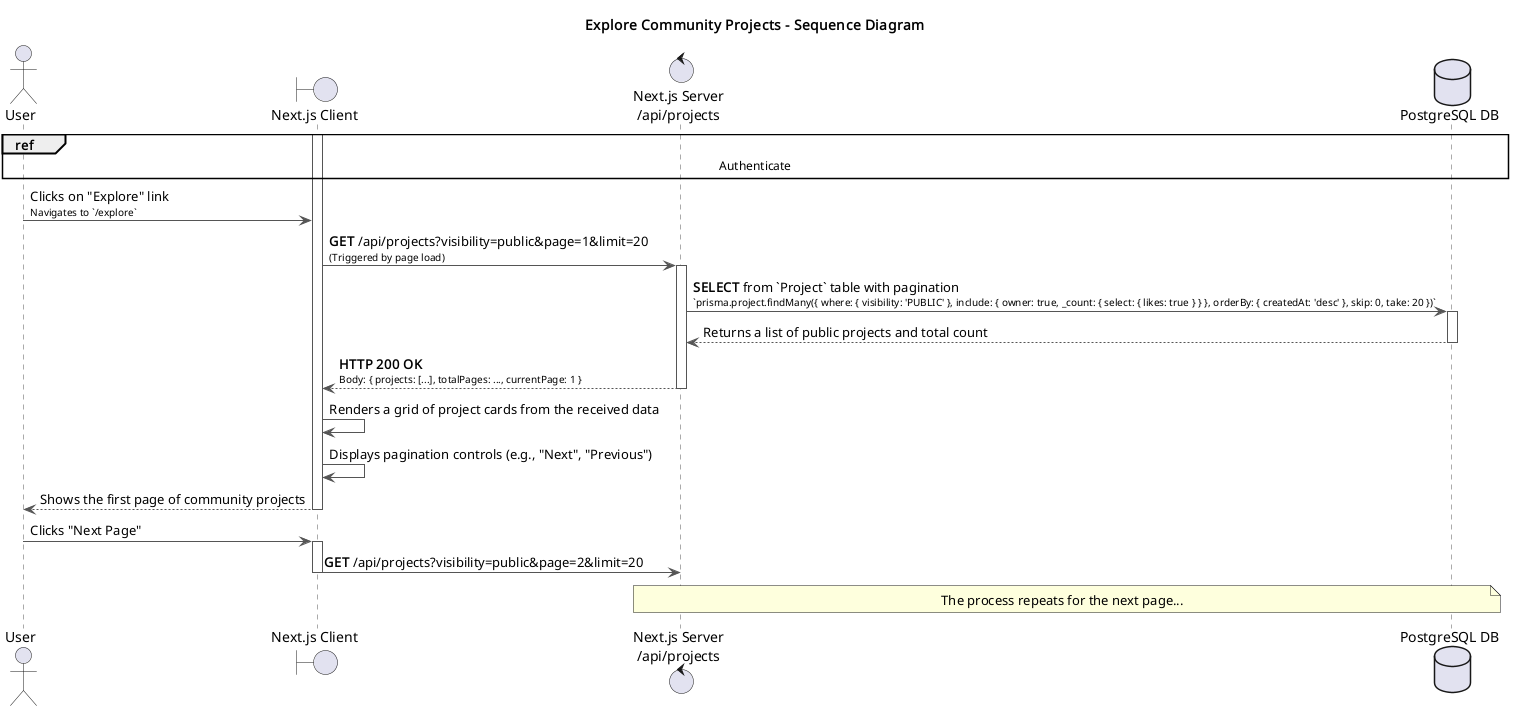
\includegraphics[width=0.85\textwidth]{conception/SprintV/sequence_diagrams/sequence_communityInteraction_6_1_ExploreCommunityAsUser.png}
\caption{Community Exploration Flow}
\label{fig:seq_explore_community}
\end{figure}

\begin{figure}[H]
\centering
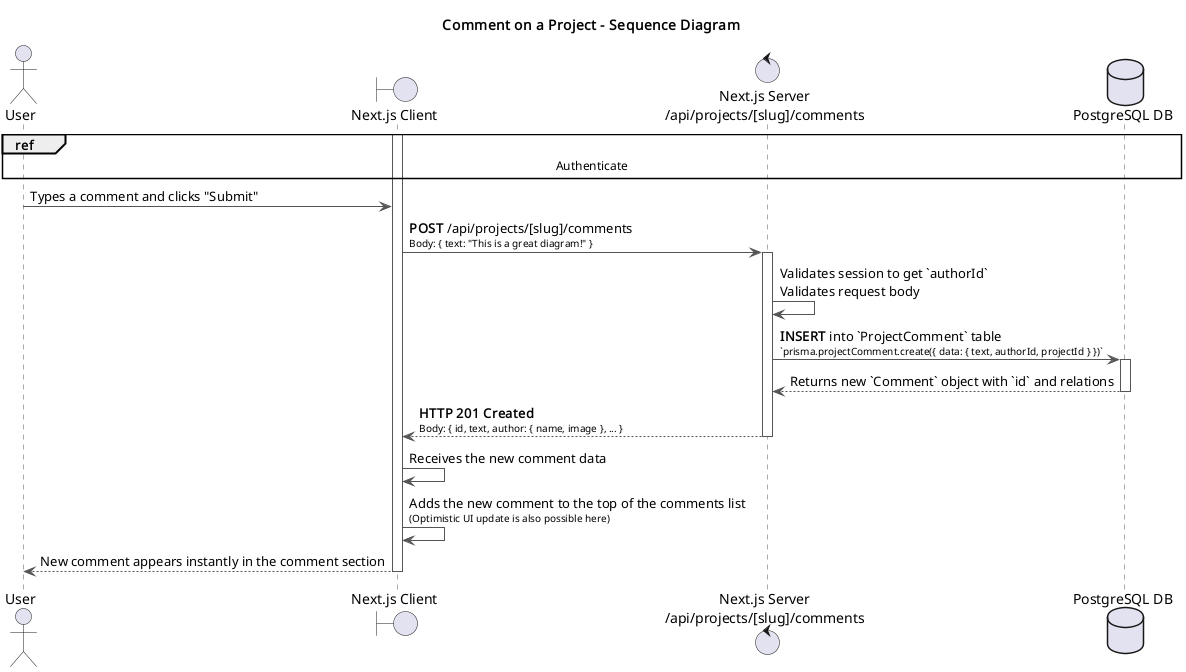
\includegraphics[width=0.85\textwidth]{conception/SprintV/sequence_diagrams/sequence_communityInteraction_6_3_CommentOnProjects.png}
\caption{Project Commenting Flow}
\label{fig:seq_comment_projects}
\end{figure}

\begin{figure}[H]
\centering
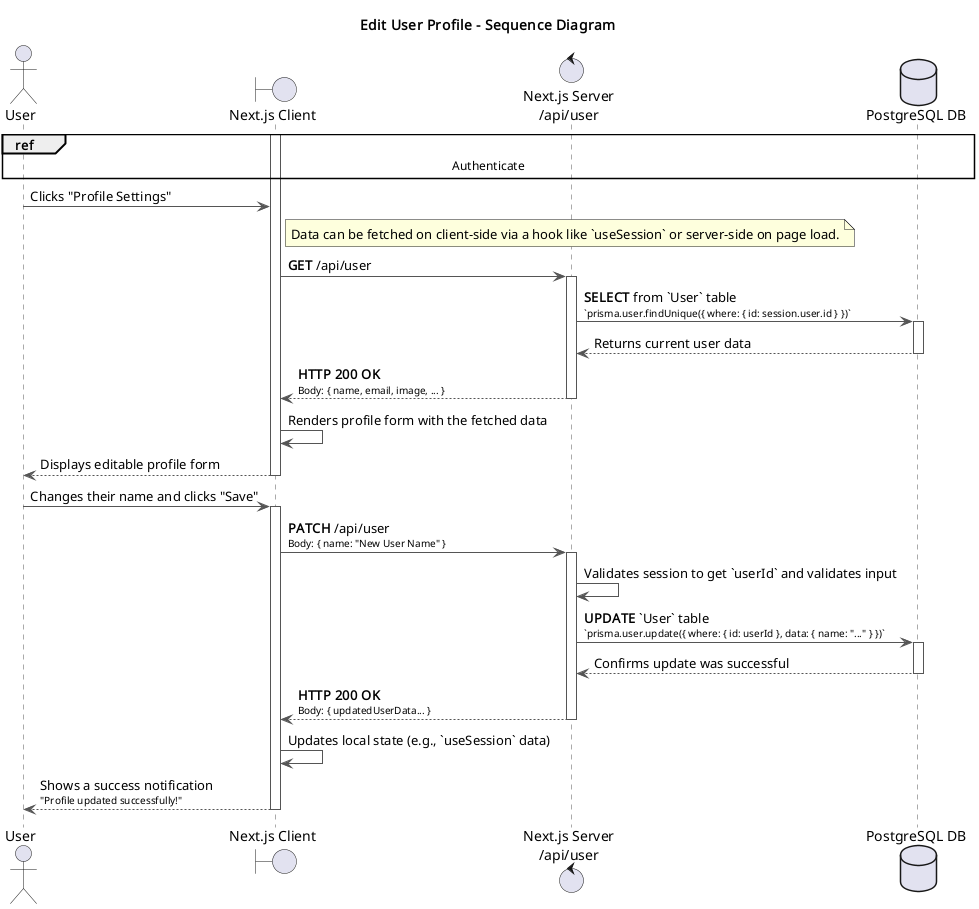
\includegraphics[width=0.75\textwidth]{conception/SprintV/sequence_diagrams/sequence_profileManagement_7_1_EditUserProfile.png}
\caption{Profile Editing Flow}
\label{fig:seq_edit_profile}
\end{figure}

\section{Implementation Results}

\subsection{Community Features}
\begin{figure}[H]
    \centering
    \includegraphics[width=0.85\textwidth]{screenshots/comment-section.png}
    \caption{Comment System Implementation}
    \label{fig:comment_section}
    \end{figure}

\begin{figure}[H]
\centering
\includegraphics[width=0.85\textwidth]{screenshots/community1.png}
\caption{Community Exploration Interface}
\label{fig:community_main}
\end{figure}




The comment system demonstrates comprehensive management including creation, editing, deletion, and interaction features for meaningful project discussions.



The profile interface enables users to maintain account information, update personal details, and manage their public platform presence with validation feedback.

\section{Sprint Retrospective}

\subsection{Achievements}
\begin{itemize}
\item Successfully implemented comprehensive community interaction features
\item Smooth integration of profile management features
\end{itemize}


\subsection{Future Actions}
\begin{itemize}
\item Implement real-time notifications for community engagement
\item Enhance mobile user experience across all features
\end{itemize}

\section{Conclusion}

Sprint 4 successfully transformed the platform into a collaborative community-driven ecosystem through comprehensive interaction features and robust profile management. The implementation of community exploration, project commenting, liking mechanisms, and profile editing establishes a solid foundation for user engagement and knowledge sharing.
